\subsubsection{UCS 5 - Modifica delle funzionalità di tracciamento dell'organizzazione}%kite level
\begin{figure}[h]
	\centering
    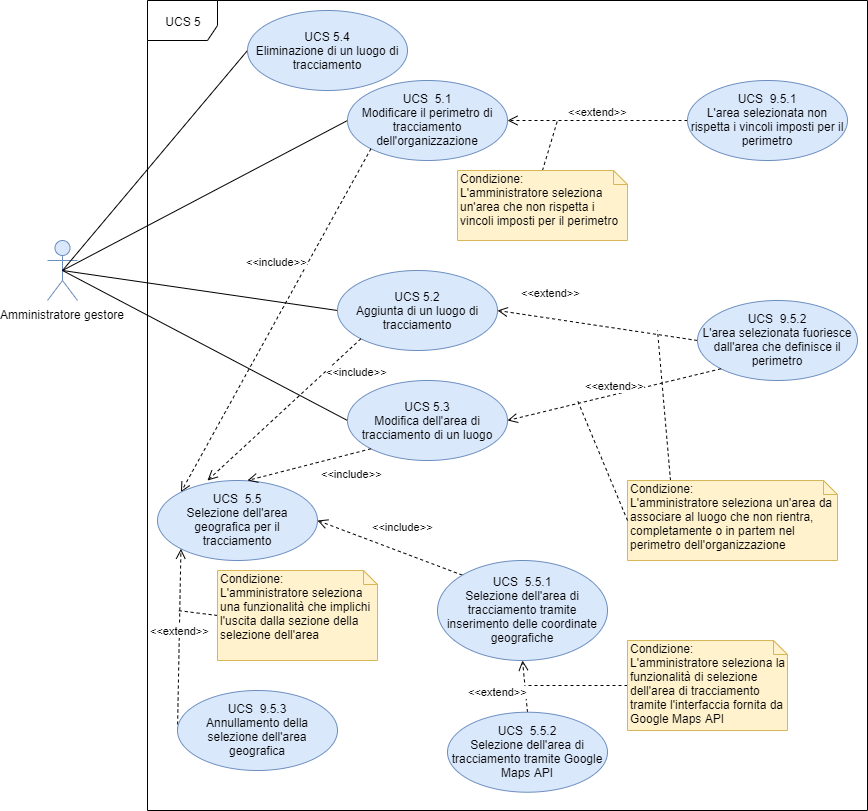
\includegraphics[scale=0.40]{sezioni/UseCase/Immagini/UCS5.png}
    \caption{UCS 5 - Modifica delle funzionalità di tracciamento dell'organizzazione}
\end{figure}
\begin{itemize}
    \item \textbf{Attori primari:} Amministratore gestore
    \item \textbf{Precondizione:} L'amministratore si trova nella sezione di modifica dei parametri dell'organizzazione.
    \item \textbf{Postcondizione:} L'amministratore ha modificato il perimetro\ap{G} e i luoghi\ap{G} per il tracciamento e ha salvato le modifiche, le quali sono state salvate nel sistema.
    \item \textbf{Scenario principale:} L'amministratore può:
    \begin{itemize}    
        \item Selezionare un nuovo perimetro\ap{G} di tracciamento dell'organizzazione [UCS 5.1];
        \item Creare dei nuovi luoghi\ap{G} di tracciamento nell'organizzazione [UCS 5.2];
        \item Modificare i luoghi\ap{G} di tracciamento dell'organizzazione [UCS 5.3];
        \item Eliminare i luoghi\ap{G} di tracciamento dell'organizzazione [UCS 5.4].
    \end{itemize}
\end{itemize}

\subsubsection{UCS 5.1 - Modificare il perimetro di tracciamento dell'organizzazione}%sea level
\begin{itemize}
    \item \textbf{Attori primari:} Amministratore gestore
    \item \textbf{Precondizione:} L'amministratore si trova nella sezione di modifica dei parametri dell'organizzazione.
    \item \textbf{Postcondizione:} L'amministratore ha modificato con successo il perimetro\ap{G} di tracciamento dell'organizzazione.
    \item \textbf{Scenario principale:} L'amministratore dovrà selezionare l'area geografica del perimetro\ap{G} da tracciare.
     \item \textbf{Scenario alternativo:} L'amministratore ha selezionato un area che non rispetta i vincoli imposti. Verrà visualizzato un messaggio d'errore [UCS 9.5.1].
    \item \textbf{Flusso di eventi:}
    \begin{enumerate}%flusso di eventi
        \item L'amministratore seleziona la funzionalità di modifica del perimetro\ap{G} di tracciamento dell'organizzazione;
        \item L'amministratore seleziona un'area geografica da associare al perimetro\ap{G} di tracciamento dell'organizzazione [UCS 5.5]. L'area selezionata deve rispettare i vincoli imposti.
    \end{enumerate}
    \item \textbf{Inclusioni:}
    \begin{enumerate}
        \item UCS 5.5 - Selezione dell'area geografica per il tracciamento.
    \end{enumerate}
    \item \textbf{Estensioni:}
    \begin{enumerate}
        \item UCS 9.5.1 - L'area selezionata non rispetta i vincoli imposti per il perimetro\ap{G}.
    \end{enumerate}
\end{itemize}

\subsubsection{UCS 5.2 - Aggiunta di un luogo di tracciamento}%sea level
\begin{itemize}
    \item \textbf{Attori primari:} Amministratore gestore
    \item \textbf{Precondizione:} L'amministratore si trova nella sezione di modifica dei parametri dell'organizzazione.
    \item \textbf{Postcondizione:} L'amministratore ha aggiunto con successo un luogo\ap{G} di tracciamento.
    \item \textbf{Scenario principale:} L'amministratore dovrà inserire i dati per il nuovo luogo\ap{G} da tracciare e l'area geografica del luogo da tracciare.
    \item \textbf{Scenario alternativo:} L'amministratore ha selezionato un area che fuoriesce dall'area che definisce il perimetro\ap{G}. Verrà visualizzato un messaggio d'errore [UCS 9.5.2].
    \item \textbf{Flusso di eventi:}
    \begin{enumerate}     
        \item L'amministratore seleziona la funzionalità per aggiungere un luogo\ap{G} di tracciamento;
        \item Inserimento del nome del luogo\ap{G} di tracciamento [UCS 5.2.1];
        \item L'amministratore seleziona un'area geografica da associare al luogo\ap{G} di tracciamento. L'area selezionata rispetta i vincoli imposti [UCS 5.5]; 
        \item L'amministratore seleziona la funzionalità per salvare le modifiche apportate.
    \end{enumerate}   
    \item \textbf{Inclusioni:}
    \begin{enumerate}
        \item UCS 5.5 - Selezione dell'area geografica per il tracciamento.
    \end{enumerate}
    \item \textbf{Estensioni:}
    \begin{enumerate}
        \item UCS 9.5.2 - L'area selezionata fuoriesce dall'area che definisce il perimetro\ap{G}.
    \end{enumerate}
\end{itemize}

\subsubsection{UCS 5.3 - Modifica dell'area di tracciamento di un luogo}%sea level
\begin{itemize}
    \item \textbf{Attori primari:} Amministratore gestore
    \item \textbf{Precondizione:} L'amministratore si trova nella sezione di modifica dei parametri\ap{G} dell'organizzazione.
    \item \textbf{Postcondizione:} L'amministratore ha modificato con successo l'area di tracciamento del luogo\ap{G}.
    \item \textbf{Scenario principale:} L'amministratore dovrà selezionare una nuova area per il tracciamento del luogo\ap{G} scelto.
    \item \textbf{Scenario alternativo:} L'amministratore ha selezionato un area che fuoriesce dall'area che definisce il perimetro\ap{G}. Verrà visualizzato un messaggio d'errore [UCS 9.5.2].
    \item \textbf{Flusso di eventi:}
    \begin{enumerate}%flusso di eventi
        \item L'amministratore seleziona la funzionalità per modificare l'area di tracciamento di un luogo\ap{G};
        \item L'amministratore seleziona il luogo\ap{G} da modificare;
        \item L'amministratore seleziona un'area geografica da associare al luogo\ap{G} di tracciamento [UCS 5.5];
        \item L'amministratore seleziona la funzionalità per salvare le modifiche apportate.
    \end{enumerate}
    \item \textbf{Inclusioni:}
    \begin{enumerate}
        \item UCS 5.5 - Selezione dell'area geografica per il tracciamento.
    \end{enumerate}
    \item \textbf{Estensioni:}
    \begin{enumerate}
        \item UCS 9.5.2 - L'area selezionata fuoriesce dall'area che definisce il perimetro\ap{G}.
    \end{enumerate}
\end{itemize}

\subsubsection{UCS 5.4 - Eliminazione di un luogo di tracciamento}%sea level
\begin{itemize}
    \item \textbf{Attori primari:} Amministratore gestore
    \item \textbf{Precondizione:} L'amministratore si trova nella sezione di modifica dei parametri\ap{G} dell'organizzazione.
    \item \textbf{Postcondizione:} L'amministratore ha modificato con successo l'area di tracciamento del luogo\ap{G}.
    \item \textbf{Scenario principale:} L'amministratore elimina un luogo\ap{G} di tracciamento definito all'interno dell'organizzazione.
    \item \textbf{Flusso di eventi:}
    \begin{enumerate}%flusso di eventi
        \item L'amministratore seleziona la funzionalità per eliminare un luogo\ap{G} dell'organizzazione;
        \item L'amministratore seleziona il luogo\ap{G} da eliminare;
        \item L'amministratore seleziona la funzionalità di conferma per rendere definitiva l'eliminazione del luogo\ap{G} di tracciamento.
    \end{enumerate}
\end{itemize}

\subsubsection{UCS 5.5 - Selezione dell'area geografica per il tracciamento}%sea level
\begin{figure}[h]
	\centering
    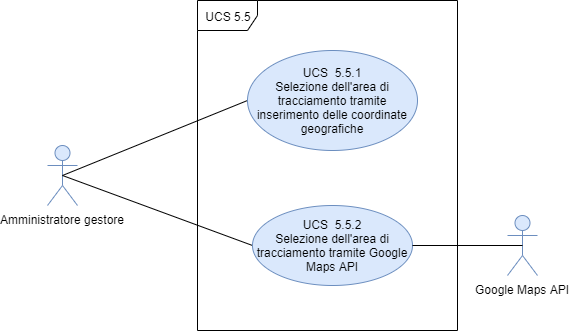
\includegraphics[scale=0.53]{sezioni/UseCase/Immagini/UCS5.5.png}
    \caption{UCS 5.5 - Selezione dell'area geografica di tracciamento}
\end{figure}
\begin{itemize}
\item \textbf{Attori primari:} Amministratore gestore
\item \textbf{Precondizione:} L'amministratore si trova nella sezione di modifica dei parametri\ap{G} dell'organizzazione.
\item \textbf{Postcondizione:} L'amministratore ha selezionato un'area per il tracciamento\ap{G}.
\item \textbf{Scenario principale:} L'amministratore deve selezionare un'area geografica per il tracciamento del luogo\ap{G} scelto.
\item \textbf{Scenario alternativo:} L'amministratore vuole uscire dalla funzionalità di selezione dell'area geografica per il tracciamento [UCS 9.5.3].
\item \textbf{Flusso di eventi:}
\begin{enumerate}
    \item L'amministratore seleziona la funzionalità di selezione dell'area;
    \item Sceglie dunque se il fine dell'area da tracciare è per un luogo\ap{G} dell'organizzazione oppure è per il perimetro\ap{G} di tracciamento;
    \item L'amministratore può scegliere se selezionare l'area inserendo le coordinate geografiche [UCS 5.5.1] oppure tramite Google Maps API [UCS 5.5.2].
\end{enumerate}
%\item \textbf{Inclusioni:}
 %   \begin{enumerate}
  %      \item UCS 5.5.1 - Selezione dell'area di tracciamento tramite inserimento delle coordinate geografiche;
   %     \item UCS 5.5.2 - Selezione dell'area di tracciamento tramite Google Maps API.
    %\end{enumerate}
\item \textbf{Estensioni:}
\begin{enumerate}
    \item UCS 5.5.3 - Annullamento della selezione dell'area geografica per il tracciamento.
\end{enumerate}
\end{itemize}

\subsubsection{UCS 5.5.1 - Selezione dell'area di tracciamento tramite inserimento delle coordinate geografiche}%fish level
\begin{itemize}
\item \textbf{Attori primari:} Amministratore gestore
\item \textbf{Precondizione:} L'amministratore si trova nella sezione di modifica dei parametri\ap{G} dell'organizzazione, in particolare nella sezione di selezione.
\item \textbf{Postcondizione:} L'amministratore ha inserito le coordinate geografiche che delimitano un'area per il tracciamento\ap{G}.
\item \textbf{Flusso di eventi:}
\begin{enumerate}
    \item L'amministratore inserisce le coordinate del primo vertice dell'area di tracciamento\ap{G};
    \item L'amministratore inserisce le coordinate del secondo vertice dell'area di tracciamento\ap{G};
    \item L'amministratore inserisce le coordinate del terzo vertice dell'area di tracciamento\ap{G};
    \item L'amministratore inserisce le coordinate del quarto vertice dell'area di tracciamento\ap{G}.
\end{enumerate}
\end{itemize}

\subsubsection{UCS 5.5.2 - Selezione dell'area di tracciamento tramite Google Maps API}%fish level
\begin{itemize}
\item \textbf{Attori primari:} Amministratore gestore
\item \textbf{Attori secondari:} Google Maps API\ap{G}
\item \textbf{Precondizione:} L'amministratore si trova nella sezione di modifica dei parametri\ap{G} dell'organizzazione, in particolare nella sezione di selezione.
\item \textbf{Postcondizione:} L'amministratore ha selezionato un'area per il tracciamento usufruendo dell'interfaccia di Google Maps API\ap{G}.
\item \textbf{Flusso di eventi:}
\begin{enumerate}
    \item L'amministratore interagisce con Google Maps API\ap{G} per selezionare l'area di tracciamento\ap{G}.
\end{enumerate}
\end{itemize}

\subsubsection{UCS 5.5.3 - Annullamento della selezione dell'area geografica per il tracciamento}%fish level
\begin{itemize}
\item \textbf{Attori primari:} Amministratore gestore
\item \textbf{Precondizione:} L'amministratore si trova nella funzionalità per la selezione dell'area geografica.
\item \textbf{Postcondizione:} L'amministratore è uscito dalla funzionalità per la selezione dell'area geografica per il tracciamento.
\item \textbf{Flusso di eventi:}
    \begin{enumerate}
    \item L'amministratore seleziona la funzionalità per l'annullamento della selezione dell'area geografica;
    \item L'amministratore conferma di voler uscire dalla funzionalità di selezione dell'area geografica.
    \end{enumerate} 
\end{itemize}